% Document setup
\documentclass[11pt]{book}

% Location of the csas-style repository: adjust path as needed
\newcommand{\locRepo}{csas-style}

% Use the style file in the csas-style repository (sr.sty)
\usepackage{\locRepo/sr}

% header-includes from R markdown entry
\usepackage{pdflscape}

% Bibliography style file
% \bibliographystyle{../csas-style/res-doc}

%%%% Commands for title page etc %%%%%

% Title
\newcommand{\rdTitle}{Evaluating the robustness of candidate management procedures in the BC sablefish (\emph{Anoplopoma fibria}) for 2019-2020.}

% French title
\newcommand{\rdTitleFr}{}

% Title short
\newcommand{\rdTitleShort}{Robustness of sablefish MPs in BC}

% Publication year
\newcommand{\rdYear}{2019}

% Publication month
\newcommand{\rdMonth}{October}

% Report number
\newcommand{\rdNumber}{nnn}

% Approver (name\\position)
\newcommand{\rdApp}{Approver Name\\
Regional Director\\
Science Branch, Pacific Region\\
Fisheries and Oceans Canada}
% \newcommand{\rdYear}{2019}
% \newcommand{\rdAppMonth}{October}
% \newcommand{\rdAppDay}{01}
\newcommand{\rdAppDate}{October 01, 2019}

% Branch
\newcommand{\rdBranch}{Science Branch}

% Region
\newcommand{\rdRegion}{Pacific Region}

% Address
\newcommand{\rdAddress}{\textsuperscript{1}Pacific Biological Station\\
Fisheries and Oceans Canada, 3190 Hammond Bay Road\\
Nanaimo, British Columbia, V9T 6N7, Canada}

% Phone
\newcommand{\rdPhone}{(250) 756-7208}

% Email
\newcommand{\rdEmail}{\href{mailto:csap@dfo-mpo.gc.ca}{\nolinkurl{csap@dfo-mpo.gc.ca}}}

%%%% End of title page commands %%%%%
\begin{document}

\MakeFirstPage

\newpage
\setcounter{table}{0}

\hypertarget{tables}{%
\section{Tables}\label{tables}}

\newpage

\begingroup\fontsize{12}{14}\selectfont
\begin{landscape}
\begin{longtable}[t]{llllllll}
\caption{\label{tab:unnamed-chunk-3}Operating model posterior distribution mean (standard deviation) biological parameter, reference point estimates, and stock status indicators for fits to the 2016 data 
and 2018 data. The columns \textbf{2016 Fit} and \textbf{2018 Fit} show the mean and standard deviation of the full posterior for the respective fits, while the remaining columns just show posterior mean values 
from the 5 stratified regions for each productivity/biomass scenario. Stock status is shown relative to unfished ($B_t/B_0$), theoretical
most productive spawning biomass ($B_t/B_{MSY}$), and the limit reference point ($B_t/(.4B_{MSY})$) for $t \in \{2016, 2018\}$. The bottom
two rows show the posterior probability of biomass being above the limit reference point in both 2016 and 2018.}\\
\toprule
\textbf{ } & \textbf{2016 Fit} & \textbf{2018 Fit} & \textbf{hiB} & \textbf{hih} & \textbf{loB} & \textbf{loh} & \textbf{mhmB}\\
\midrule
\endfirsthead
\caption*{}\\
\toprule
\textbf{ } & \textbf{2016 Fit} & \textbf{2018 Fit} & \textbf{hiB} & \textbf{hih} & \textbf{loB} & \textbf{loh} & \textbf{mhmB}\\
\midrule
\endhead
\
\endfoot
\bottomrule
\endlastfoot
$B_0$ & 57 (1.3) & 54.1 (3.3) & 55.6 & 53.9 & 52.2 & 54.2 & 54\\
$M_m$ & 0.0411 (0.00027) & 0.0421 (0.0026) & 0.0425 & 0.0419 & 0.0412 & 0.0422 & 0.042\\
$M_f$ & 0.0788 (0.0014) & 0.0877 (0.0025) & 0.087 & 0.0874 & 0.0879 & 0.0879 & 0.0876\\
$h$ & 0.556 (0.064) & 0.617 (0.062) & 0.62 & 0.689 & 0.617 & 0.545 & 0.618\\
$B_{2016}$ & 10.9 (1.2) & 12.5 (1.4) & 14 & 12.4 & 11 & 12.5 & 12.5\\
$B_{2018}$ &  & 16.3 (2) & 18.6 & 16.2 & 14.1 & 16.4 & 16.3\\
$B_{MSY}$ & 23.4 (0.96) & 20.4 (1.7) & 20.9 & 18.9 & 19.8 & 21.9 & 20.4\\
$U_{MSY}$ & 0.0433 (0.0062) & 0.0734 (0.01) & 0.0736 & 0.0853 & 0.0729 & 0.0619 & 0.0733\\
Legal $U_{MSY}$ & 0.0423 (0.006) & 0.0773 (0.011) & 0.0775 & 0.0902 & 0.0766 & 0.0647 & 0.0771\\
$MSY$ & 2.79 (0.27) & 4.37 (0.45) & 4.46 & 4.75 & 4.27 & 3.98 & 4.38\\
$B_{2016}/B_0$ & 0.191 (0.018) & 0.231 (0.021) & 0.253 & 0.231 & 0.212 & 0.232 & 0.231\\
$B_{2016}/B_{MSY}$ & 0.467 (0.049) & 0.613 (0.065) & 0.673 & 0.66 & 0.558 & 0.573 & 0.612\\
$B_{2016}/(.4B_{MSY})$ & 1.17 (0.12) & 1.53 (0.16) & 1.68 & 1.65 & 1.39 & 1.43 & 1.53\\
$B_{2018}/B_0$ &  & 0.301 (0.032) & 0.335 & 0.301 & 0.271 & 0.304 & 0.302\\
$B_{2018}/B_{MSY}$ &  & 0.8 (0.096) & 0.891 & 0.86 & 0.714 & 0.75 & 0.799\\
$B_{2018}/(.4B_{MSY})$ &  & 2 (0.24) & 2.23 & 2.15 & 1.79 & 1.88 & 2\\
$P(B_{2016} \geq .4B_{MSY})$ & 0.93 & 1 &  &  &  &  & \\
$P(B_{2018} \geq .4B_{MSY})$ &  & 1 &  &  &  &  & \\*
\end{longtable}
\end{landscape}
\endgroup{}

\newpage

\begingroup\fontsize{9}{11}\selectfont
\begin{landscape}
\begin{longtable}[t]{llccccccccc}
\caption{\label{tab:unnamed-chunk-5}Weighted performance metrics for all candidate management procedures on the reference set of operating models, where recruitment is taken from the OM estimate for the 2015 year class. Conservation performance metrics that pass the criteria in the header are indicated by a bullet. Catch is given in biomass units, which are measured in kilotonnes. Table is sorted by 10 year average catch $\bar{C}_{2019:2028}$. For Objective 2, Obs refers to the observed probability of decline, and Acc to the acceptable probability of decline, linearly interpolated between 0.05 at $0.4B_{MSY}$ and 0.5 at $B_{MSY}$.}\\
\toprule
\multicolumn{2}{c}{\textbf{ }} & \multicolumn{1}{c}{\textbf{Objective 1}} & \multicolumn{1}{c}{\textbf{Objective 2}} & \multicolumn{1}{c}{\textbf{Objective 3}} & \multicolumn{1}{c}{\textbf{Objective 4}} & \multicolumn{1}{c}{\textbf{Objective 5}} & \multicolumn{4}{c}{\textbf{Other Important Quantities}} \\
\cmidrule(l{3pt}r{3pt}){3-3} \cmidrule(l{3pt}r{3pt}){4-4} \cmidrule(l{3pt}r{3pt}){5-5} \cmidrule(l{3pt}r{3pt}){6-6} \cmidrule(l{3pt}r{3pt}){7-7} \cmidrule(l{3pt}r{3pt}){8-11}
\multicolumn{2}{c}{\textbf{ }} & \multicolumn{1}{c}{\textbf{P > .95}} & \multicolumn{1}{c}{\textbf{Obs < Acc}} & \multicolumn{1}{c}{\textbf{P > .5}} & \multicolumn{1}{c}{\textbf{min}} & \multicolumn{1}{c}{\textbf{max}} & \multicolumn{4}{c}{\textbf{ }} \\
\cmidrule(l{3pt}r{3pt}){3-3} \cmidrule(l{3pt}r{3pt}){4-4} \cmidrule(l{3pt}r{3pt}){5-5} \cmidrule(l{3pt}r{3pt}){6-6} \cmidrule(l{3pt}r{3pt}){7-7}
\textbf{No.} & \textbf{MP Label} & \textbf{$P(B_t \geq .4B_{MSY})$} & \textbf{$P(Decline)$} & \textbf{$P(B_{2052} > B_{MSY})$} & \textbf{$P(C_t < 1.992)$} & \textbf{$\bar{C}_{2019:2028}$} & \textbf{$AAV$} & \textbf{$C_{2019}$} & \textbf{$B_{2019}/B0$} & \textbf{$F_{2022}$}\\
\midrule
\endfirsthead
\caption*{}\\
\toprule
\textbf{No.} & \textbf{MP Label} & \textbf{$P(B_t \geq .4B_{MSY})$} & \textbf{$P(Decline)$} & \textbf{$P(B_{2052} > B_{MSY})$} & \textbf{$P(C_t < 1.992)$} & \textbf{$\bar{C}_{2019:2028}$} & \textbf{$AAV$} & \textbf{$C_{2019}$} & \textbf{$B_{2019}/B0$} & \textbf{$F_{2022}$}\\
\midrule
\endhead
\
\endfoot
\bottomrule
\endlastfoot
14 & NSL & $\bullet$ & $\bullet$ & $\bullet$ & 0.01 & 4.510 & 8 & 3.39 & 0.35 & 0.0738\\
17 & cap0\_am5 & $\bullet$ & $\bullet$ & $\bullet$ & 0.02 & 4.112 & 8 & 3.39 & 0.35 & 0.0783\\
3 & cap.5\_hstAl\_am5 & $\bullet$ & $\bullet$ & $\bullet$ & 0.02 & 4.005 & 8 & 3.39 & 0.35 & 0.0728\\
16 & cap0\_am10 & $\bullet$ & $\bullet$ & $\bullet$ & 0.02 & 4.005 & 8 & 3.39 & 0.35 & 0.0699\\
5 & cap.5\_rctAl\_am5 & $\bullet$ & $\bullet$ & $\bullet$ & 0.02 & 3.930 & 8 & 3.39 & 0.35 & 0.0712\\
7 & cap1.0\_hstAl\_am5 & $\bullet$ & $\bullet$ & $\bullet$ & 0.02 & 3.927 & 8 & 3.39 & 0.35 & 0.0680\\
2 & cap.5\_hstAl\_am10 & $\bullet$ & $\bullet$ & $\bullet$ & 0.02 & 3.921 & 8 & 3.39 & 0.35 & 0.0665\\
4 & cap.5\_rctAl\_am10 & $\bullet$ & $\bullet$ & $\bullet$ & 0.02 & 3.864 & 8 & 3.39 & 0.35 & 0.0654\\
6 & cap1.0\_hstAl\_am10 & $\bullet$ & $\bullet$ & $\bullet$ & 0.02 & 3.850 & 8 & 3.39 & 0.35 & 0.0636\\
11 & cap1.5\_hstAl\_am5 & $\bullet$ & $\bullet$ & $\bullet$ & 0.02 & 3.842 & 8 & 3.39 & 0.35 & 0.0638\\
10 & cap1.5\_hstAl\_am10 & $\bullet$ & $\bullet$ & $\bullet$ & 0.02 & 3.804 & 8 & 3.39 & 0.35 & 0.0613\\
8 & cap1.0\_rctAl\_am10 & $\bullet$ & $\bullet$ & $\bullet$ & 0.03 & 3.782 & 8 & 3.39 & 0.35 & 0.0624\\
9 & cap1.0\_rctAl\_am5 & $\bullet$ & $\bullet$ & $\bullet$ & 0.02 & 3.767 & 8 & 3.39 & 0.35 & 0.0651\\
15 & noCap & $\bullet$ & $\bullet$ & $\bullet$ & 0.03 & 3.729 & 7 & 3.39 & 0.35 & 0.0582\\
12 & cap1.5\_rctAl\_am10 & $\bullet$ & $\bullet$ & $\bullet$ & 0.03 & 3.721 & 8 & 3.39 & 0.35 & 0.0603\\
13 & cap1.5\_rctAl\_am5 & $\bullet$ & $\bullet$ & $\bullet$ & 0.02 & 3.702 & 8 & 3.39 & 0.35 & 0.0621\\
1 & NoFish & $\bullet$ & $\bullet$ & $\bullet$ & 1.00 & 0.000 & 0 & 0.00 & 0.35 & 0.0550\\*
\end{longtable}
\end{landscape}
\endgroup{}

\newpage

\begingroup\fontsize{12}{14}\selectfont
\begin{longtable}[t]{lr}
\caption{\label{tab:unnamed-chunk-7}Price per pound of sablefish in each weight class. Weight classes are defined by the limits of that class, in pounds (e.g., 2/3 is the class of fish between 2 and 3 pounds).}\\
\toprule
\textbf{Weight Class (lb)} & \textbf{Price (\$/lb)}\\
\midrule
0/2 & 6.0\\
2/3 & 7.7\\
3/4 & 8.0\\
4/5 & 9.0\\
5/7 & 11.0\\
7+ & 12.0\\
\bottomrule
\end{longtable}
\endgroup{}

\newpage

\begingroup\fontsize{12}{14}\selectfont
\begin{landscape}
\begin{longtable}[t]{llcccccccccl}
\caption{\label{tab:unnamed-chunk-8}Weighted economic performance metrics for the first 10 years of the projections in the reference OM set. Column 3 shows the average catch over the first 10 years, and the remaining columns show the total value (\$m) of catch $C$ and discards $D$ for all sectors, and the yearly average income $I$ in dollars per tonne of catch, over the next 10 years. All values are taken at 4 significant figures. Table is sorted by 10 year average catch $\bar{C}_{2019:2028}$.}\\
\toprule
\multicolumn{2}{c}{\textbf{ }} & \multicolumn{1}{c}{\textbf{Av. Catch (kt)}} & \multicolumn{6}{c}{\textbf{10 year revenue (\$ millions)}} & \multicolumn{3}{c}{\textbf{Av. revenue (\$/t)}} \\
\cmidrule(l{3pt}r{3pt}){3-3} \cmidrule(l{3pt}r{3pt}){4-9} \cmidrule(l{3pt}r{3pt}){10-12}
\textbf{No.} & \textbf{MP Label} & \textbf{$\bar{C}_{2019:2028}$} & \textbf{$C^{trap}$} & \textbf{$C^{hook}$} & \textbf{$C^{trawl}$} & \textbf{$D^{trap}$} & \textbf{$D^{hook}$} & \textbf{$D^{trawl}$} & \textbf{$R^{trap}$} & \textbf{$R^{hook}$} & \textbf{$R^{trawl}$}\\
\midrule
\endfirsthead
\caption*{}\\
\toprule
\textbf{No.} & \textbf{MP Label} & \textbf{$\bar{C}_{2019:2028}$} & \textbf{$C^{trap}$} & \textbf{$C^{hook}$} & \textbf{$C^{trawl}$} & \textbf{$D^{trap}$} & \textbf{$D^{hook}$} & \textbf{$D^{trawl}$} & \textbf{$R^{trap}$} & \textbf{$R^{hook}$} & \textbf{$R^{trawl}$}\\
\midrule
\endhead
\
\endfoot
\bottomrule
\endlastfoot
14 & NSL & 4.510 & 417.6 & 335.4 & 60.81 & 0.000 & 0.00 & 0.00 & 17970 & 18320 & 16270\\
17 & cap0\_am5 & 4.112 & 385.7 & 321.0 & 42.67 & 10.950 & 13.45 & 25.81 & 18130 & 18340 & 17320\\
3 & cap.5\_hstAl\_am5 & 4.005 & 370.9 & 312.5 & 46.34 & 10.550 & 13.08 & 27.75 & 18130 & 18340 & 17330\\
16 & cap0\_am10 & 4.005 & 375.1 & 306.2 & 47.97 & 10.680 & 12.83 & 28.92 & 18130 & 18340 & 17330\\
5 & cap.5\_rctAl\_am5 & 3.930 & 362.8 & 302.2 & 50.54 & 10.320 & 12.65 & 29.97 & 18140 & 18340 & 17330\\
7 & cap1.0\_hstAl\_am5 & 3.927 & 358.3 & 305.8 & 50.07 & 10.210 & 12.78 & 29.71 & 18140 & 18340 & 17330\\
2 & cap.5\_hstAl\_am10 & 3.921 & 364.1 & 299.3 & 49.78 & 10.400 & 12.53 & 29.86 & 18130 & 18340 & 17330\\
4 & cap.5\_rctAl\_am10 & 3.864 & 358.6 & 292.9 & 52.15 & 10.240 & 12.27 & 31.12 & 18140 & 18340 & 17340\\
6 & cap1.0\_hstAl\_am10 & 3.850 & 355.3 & 294.0 & 51.77 & 10.160 & 12.31 & 30.90 & 18140 & 18340 & 17340\\
11 & cap1.5\_hstAl\_am5 & 3.842 & 348.0 & 298.1 & 52.75 & 9.943 & 12.46 & 31.14 & 18140 & 18340 & 17340\\
10 & cap1.5\_hstAl\_am10 & 3.804 & 349.1 & 289.1 & 53.25 & 10.000 & 12.11 & 31.70 & 18140 & 18340 & 17340\\
8 & cap1.0\_rctAl\_am10 & 3.782 & 348.5 & 284.7 & 55.07 & 9.982 & 11.93 & 32.71 & 18140 & 18340 & 17340\\
9 & cap1.0\_rctAl\_am5 & 3.767 & 343.6 & 286.5 & 55.58 & 9.818 & 12.00 & 32.67 & 18140 & 18340 & 17340\\
15 & noCap & 3.729 & 347.9 & 277.5 & 53.58 & 10.010 & 11.66 & 32.11 & 18140 & 18340 & 17340\\
12 & cap1.5\_rctAl\_am10 & 3.721 & 342.4 & 279.8 & 54.97 & 9.830 & 11.73 & 32.73 & 18140 & 18340 & 17340\\
13 & cap1.5\_rctAl\_am5 & 3.702 & 336.7 & 280.8 & 56.10 & 9.642 & 11.76 & 33.18 & 18140 & 18340 & 17340\\
1 & NoFish & 0.000 & 0.0 & 0.0 & 0.00 & 0.000 & 0.00 & 0.00 & 0 & 0 & 0\\*
\end{longtable}
\end{landscape}
\endgroup{}

\newpage

\begingroup\fontsize{9}{11}\selectfont
\begin{landscape}
\begin{longtable}[t]{llccccccccc}
\caption{\label{tab:unnamed-chunk-9}Weighted performance metrics for all candidate management procedures on the robustness set of operating models, where recruitment is simulated stochastically off the stock-recruit curve for the 2015 year class. Conservation performance metrics that pass the criteria in the header are indicated by a bullet. Catch is given in biomass units, which are measured in kilotonnes. Table is sorted by 10 year average catch $\bar{C}_{2019:2028}$. For Objective 2, Obs refers to the observed probability of decline, and Acc to the acceptable probability of decline, linearly interpolated between 0.05 at $0.4B_{MSY}$ and 0.5 at $B_{MSY}$.}\\
\toprule
\multicolumn{2}{c}{\textbf{ }} & \multicolumn{1}{c}{\textbf{Objective 1}} & \multicolumn{1}{c}{\textbf{Objective 2}} & \multicolumn{1}{c}{\textbf{Objective 3}} & \multicolumn{1}{c}{\textbf{Objective 4}} & \multicolumn{1}{c}{\textbf{Objective 5}} & \multicolumn{4}{c}{\textbf{Other Important Quantities}} \\
\cmidrule(l{3pt}r{3pt}){3-3} \cmidrule(l{3pt}r{3pt}){4-4} \cmidrule(l{3pt}r{3pt}){5-5} \cmidrule(l{3pt}r{3pt}){6-6} \cmidrule(l{3pt}r{3pt}){7-7} \cmidrule(l{3pt}r{3pt}){8-11}
\multicolumn{2}{c}{\textbf{ }} & \multicolumn{1}{c}{\textbf{P > .95}} & \multicolumn{1}{c}{\textbf{Obs < Acc}} & \multicolumn{1}{c}{\textbf{P > .5}} & \multicolumn{1}{c}{\textbf{min}} & \multicolumn{1}{c}{\textbf{max}} & \multicolumn{4}{c}{\textbf{ }} \\
\cmidrule(l{3pt}r{3pt}){3-3} \cmidrule(l{3pt}r{3pt}){4-4} \cmidrule(l{3pt}r{3pt}){5-5} \cmidrule(l{3pt}r{3pt}){6-6} \cmidrule(l{3pt}r{3pt}){7-7}
\textbf{No.} & \textbf{MP Label} & \textbf{$P(B_t \geq .4B_{MSY})$} & \textbf{$P(Decline)$} & \textbf{$P(B_{2052} > B_{MSY})$} & \textbf{$P(C_t < 1.992)$} & \textbf{$\bar{C}_{2019:2028}$} & \textbf{$AAV$} & \textbf{$C_{2019}$} & \textbf{$B_{2019}/B0$} & \textbf{$F_{2022}$}\\
\midrule
\endfirsthead
\caption*{}\\
\toprule
\textbf{No.} & \textbf{MP Label} & \textbf{$P(B_t \geq .4B_{MSY})$} & \textbf{$P(Decline)$} & \textbf{$P(B_{2052} > B_{MSY})$} & \textbf{$P(C_t < 1.992)$} & \textbf{$\bar{C}_{2019:2028}$} & \textbf{$AAV$} & \textbf{$C_{2019}$} & \textbf{$B_{2019}/B0$} & \textbf{$F_{2022}$}\\
\midrule
\endhead
\
\endfoot
\bottomrule
\endlastfoot
14 & NSL & $\bullet$ & $\bullet$ & $\bullet$ & 0.08 & 2.767 & 11 & 3.39 & 0.24 & 0.0674\\
17 & cap0\_am5 & $\bullet$ & $\bullet$ & $\bullet$ & 0.15 & 2.505 & 14 & 3.40 & 0.24 & 0.0719\\
3 & cap.5\_hstAl\_am5 & $\bullet$ & $\bullet$ & $\bullet$ & 0.18 & 2.440 & 15 & 3.40 & 0.24 & 0.0643\\
16 & cap0\_am10 & $\bullet$ & $\bullet$ & $\bullet$ & 0.18 & 2.435 & 15 & 3.40 & 0.24 & 0.0635\\
7 & cap1.0\_hstAl\_am5 & $\bullet$ & $0.27>0.26$ & $\bullet$ & 0.20 & 2.392 & 15 & 3.40 & 0.24 & 0.0589\\
2 & cap.5\_hstAl\_am10 & $\bullet$ & $\bullet$ & $\bullet$ & 0.21 & 2.385 & 15 & 3.40 & 0.24 & 0.0592\\
5 & cap.5\_rctAl\_am5 & $\bullet$ & $\bullet$ & $\bullet$ & 0.21 & 2.377 & 15 & 3.40 & 0.24 & 0.0622\\
6 & cap1.0\_hstAl\_am10 & $\bullet$ & $\bullet$ & $\bullet$ & 0.22 & 2.364 & 15 & 3.40 & 0.24 & 0.0564\\
11 & cap1.5\_hstAl\_am5 & $\bullet$ & $0.27>0.26$ & $\bullet$ & 0.22 & 2.358 & 14 & 3.40 & 0.24 & 0.0556\\
4 & cap.5\_rctAl\_am10 & $\bullet$ & $\bullet$ & $\bullet$ & 0.23 & 2.349 & 15 & 3.40 & 0.24 & 0.0580\\
10 & cap1.5\_hstAl\_am10 & $\bullet$ & $\bullet$ & $\bullet$ & 0.24 & 2.340 & 14 & 3.40 & 0.24 & 0.0543\\
12 & cap1.5\_rctAl\_am10 & $\bullet$ & $\bullet$ & $\bullet$ & 0.24 & 2.322 & 15 & 3.40 & 0.24 & 0.0540\\
8 & cap1.0\_rctAl\_am10 & $\bullet$ & $\bullet$ & $\bullet$ & 0.24 & 2.322 & 15 & 3.40 & 0.24 & 0.0552\\
13 & cap1.5\_rctAl\_am5 & $\bullet$ & $\bullet$ & $\bullet$ & 0.24 & 2.312 & 15 & 3.40 & 0.24 & 0.0546\\
9 & cap1.0\_rctAl\_am5 & $\bullet$ & $\bullet$ & $\bullet$ & 0.24 & 2.309 & 16 & 3.40 & 0.24 & 0.0567\\
15 & noCap & $\bullet$ & $\bullet$ & $\bullet$ & 0.25 & 2.305 & 14 & 3.40 & 0.24 & 0.0524\\
1 & NoFish & $\bullet$ & $\bullet$ & $\bullet$ & 1.00 & 0.000 & 0 & 0.00 & 0.24 & 0.0550\\*
\end{longtable}
\end{landscape}
\endgroup{}

\newpage

\begingroup\fontsize{12}{14}\selectfont
\begin{landscape}
\begin{longtable}[t]{llcccccccccl}
\caption{\label{tab:unnamed-chunk-10}Weighted economic performance metrics for the first 10 years of the projections in the robustness OM set. Column 3 shows the average catch over the first 10 years, and the remaining columns show the total value (\$m) of catch $C$ and discards $D$ for all sectors, and the yearly average income $I$ in dollars per tonne of catch, over the next 10 years. All values are taken at 4 significant figures. Table is sorted by 10 year average catch $\bar{C}_{2019:2028}$.}\\
\toprule
\multicolumn{2}{c}{\textbf{ }} & \multicolumn{1}{c}{\textbf{Av. Catch (kt)}} & \multicolumn{6}{c}{\textbf{10 year revenue (\$ millions)}} & \multicolumn{3}{c}{\textbf{Av. revenue (\$/t)}} \\
\cmidrule(l{3pt}r{3pt}){3-3} \cmidrule(l{3pt}r{3pt}){4-9} \cmidrule(l{3pt}r{3pt}){10-12}
\textbf{No.} & \textbf{MP Label} & \textbf{$\bar{C}_{2019:2028}$} & \textbf{$C^{trap}$} & \textbf{$C^{hook}$} & \textbf{$C^{trawl}$} & \textbf{$D^{trap}$} & \textbf{$D^{hook}$} & \textbf{$D^{trawl}$} & \textbf{$R^{trap}$} & \textbf{$R^{hook}$} & \textbf{$R^{trawl}$}\\
\midrule
\endfirsthead
\caption*{}\\
\toprule
\textbf{No.} & \textbf{MP Label} & \textbf{$\bar{C}_{2019:2028}$} & \textbf{$C^{trap}$} & \textbf{$C^{hook}$} & \textbf{$C^{trawl}$} & \textbf{$D^{trap}$} & \textbf{$D^{hook}$} & \textbf{$D^{trawl}$} & \textbf{$R^{trap}$} & \textbf{$R^{hook}$} & \textbf{$R^{trawl}$}\\
\midrule
\endhead
\
\endfoot
\bottomrule
\endlastfoot
14 & NSL & 2.767 & 256.2 & 205.8 & 36.44 & 0.000 & 0.000 & 0.00 & 18030 & 18340 & 15880\\
17 & cap0\_am5 & 2.505 & 237.6 & 195.3 & 22.96 & 6.304 & 8.055 & 17.00 & 18190 & 18360 & 17170\\
3 & cap.5\_hstAl\_am5 & 2.440 & 226.8 & 189.8 & 26.25 & 5.976 & 7.804 & 19.56 & 18200 & 18370 & 17220\\
16 & cap0\_am10 & 2.435 & 229.9 & 186.1 & 26.50 & 6.061 & 7.657 & 20.09 & 18200 & 18360 & 17210\\
7 & cap1.0\_hstAl\_am5 & 2.392 & 220.4 & 184.6 & 29.42 & 5.778 & 7.571 & 22.07 & 18200 & 18370 & 17230\\
2 & cap.5\_hstAl\_am10 & 2.385 & 223.0 & 182.3 & 28.56 & 5.853 & 7.482 & 21.69 & 18200 & 18370 & 17230\\
5 & cap.5\_rctAl\_am5 & 2.377 & 220.6 & 181.0 & 29.58 & 5.776 & 7.426 & 22.12 & 18200 & 18370 & 17230\\
6 & cap1.0\_hstAl\_am10 & 2.364 & 219.4 & 179.3 & 30.70 & 5.741 & 7.351 & 23.39 & 18200 & 18370 & 17240\\
11 & cap1.5\_hstAl\_am5 & 2.358 & 218.2 & 178.0 & 31.63 & 5.696 & 7.292 & 23.92 & 18200 & 18370 & 17240\\
4 & cap.5\_rctAl\_am10 & 2.349 & 219.3 & 177.4 & 30.72 & 5.735 & 7.274 & 23.37 & 18200 & 18370 & 17240\\
10 & cap1.5\_hstAl\_am10 & 2.340 & 217.2 & 175.1 & 32.03 & 5.670 & 7.176 & 24.50 & 18210 & 18370 & 17240\\
12 & cap1.5\_rctAl\_am10 & 2.322 & 214.6 & 173.2 & 33.28 & 5.590 & 7.083 & 25.58 & 18210 & 18370 & 17240\\
8 & cap1.0\_rctAl\_am10 & 2.322 & 215.0 & 173.8 & 33.06 & 5.605 & 7.114 & 25.30 & 18210 & 18370 & 17240\\
13 & cap1.5\_rctAl\_am5 & 2.312 & 212.5 & 173.4 & 33.49 & 5.526 & 7.091 & 25.62 & 18210 & 18370 & 17240\\
9 & cap1.0\_rctAl\_am5 & 2.309 & 212.7 & 174.3 & 33.22 & 5.537 & 7.131 & 25.16 & 18210 & 18370 & 17250\\
15 & noCap & 2.305 & 214.7 & 171.1 & 32.79 & 5.600 & 7.004 & 25.31 & 18210 & 18370 & 17240\\
1 & NoFish & 0.000 & 0.0 & 0.0 & 0.00 & 0.000 & 0.000 & 0.00 & 0 & 0 & 0\\*
\end{longtable}
\end{landscape}
\endgroup{}

\newpage

\begingroup\fontsize{9}{11}\selectfont
\begin{landscape}
\begin{longtable}[t]{llccccccccc}
\caption{\label{tab:unnamed-chunk-12}Weighted performance metrics for all candidate management procedures, with harvest rates tuned to performance on the reference set of operating models, and applied to the robustness set of operating models where recruitment is simulated stochastically off the stock-recruit curve for the 2015 year class. Conservation performance metrics that pass the criteria in the header are indicated by a bullet. Catch is given in biomass units, which are measured in kilotonnes. Table is sorted by 10 year average catch $\bar{C}_{2019:2028}$. For Objective 2, Obs refers to the observed probability of decline, and Acc to the acceptable probability of decline, linearly interpolated between 0.05 at $0.4B_{MSY}$ and 0.5 at $B_{MSY}$.}\\
\toprule
\multicolumn{2}{c}{\textbf{ }} & \multicolumn{1}{c}{\textbf{Objective 1}} & \multicolumn{1}{c}{\textbf{Objective 2}} & \multicolumn{1}{c}{\textbf{Objective 3}} & \multicolumn{1}{c}{\textbf{Objective 4}} & \multicolumn{1}{c}{\textbf{Objective 5}} & \multicolumn{4}{c}{\textbf{Other Important Quantities}} \\
\cmidrule(l{3pt}r{3pt}){3-3} \cmidrule(l{3pt}r{3pt}){4-4} \cmidrule(l{3pt}r{3pt}){5-5} \cmidrule(l{3pt}r{3pt}){6-6} \cmidrule(l{3pt}r{3pt}){7-7} \cmidrule(l{3pt}r{3pt}){8-11}
\multicolumn{2}{c}{\textbf{ }} & \multicolumn{1}{c}{\textbf{P > .95}} & \multicolumn{1}{c}{\textbf{Obs < Acc}} & \multicolumn{1}{c}{\textbf{P > .5}} & \multicolumn{1}{c}{\textbf{min}} & \multicolumn{1}{c}{\textbf{max}} & \multicolumn{4}{c}{\textbf{ }} \\
\cmidrule(l{3pt}r{3pt}){3-3} \cmidrule(l{3pt}r{3pt}){4-4} \cmidrule(l{3pt}r{3pt}){5-5} \cmidrule(l{3pt}r{3pt}){6-6} \cmidrule(l{3pt}r{3pt}){7-7}
\textbf{No.} & \textbf{MP Label} & \textbf{$P(B_t \geq .4B_{MSY})$} & \textbf{$P(Decline)$} & \textbf{$P(B_{2052} > B_{MSY})$} & \textbf{$P(C_t < 1.992)$} & \textbf{$\bar{C}_{2019:2028}$} & \textbf{$AAV$} & \textbf{$C_{2019}$} & \textbf{$B_{2019}/B0$} & \textbf{$F_{2022}$}\\
\midrule
\endfirsthead
\caption*{}\\
\toprule
\textbf{No.} & \textbf{MP Label} & \textbf{$P(B_t \geq .4B_{MSY})$} & \textbf{$P(Decline)$} & \textbf{$P(B_{2052} > B_{MSY})$} & \textbf{$P(C_t < 1.992)$} & \textbf{$\bar{C}_{2019:2028}$} & \textbf{$AAV$} & \textbf{$C_{2019}$} & \textbf{$B_{2019}/B0$} & \textbf{$F_{2022}$}\\
\midrule
\endhead
\
\endfoot
\bottomrule
\endlastfoot
14 & NSL & $\bullet$ & $\bullet$ & $0.42<0.5$ & 0.09 & 2.920 & 11 & 3.39 & 0.24 & 0.0738\\
17 & cap0\_am5 & $\bullet$ & $0.3>0.26$ & $0.42<0.5$ & 0.13 & 2.632 & 14 & 3.40 & 0.24 & 0.0783\\
3 & cap.5\_hstAl\_am5 & $\bullet$ & $0.32>0.26$ & $0.41<0.5$ & 0.14 & 2.612 & 14 & 3.40 & 0.24 & 0.0728\\
7 & cap1.0\_hstAl\_am5 & $\bullet$ & $0.34>0.26$ & $0.4<0.5$ & 0.15 & 2.589 & 14 & 3.40 & 0.24 & 0.0680\\
16 & cap0\_am10 & $\bullet$ & $0.32>0.26$ & $0.41<0.5$ & 0.15 & 2.573 & 14 & 3.40 & 0.24 & 0.0699\\
5 & cap.5\_rctAl\_am5 & $\bullet$ & $0.33>0.26$ & $0.4<0.5$ & 0.16 & 2.558 & 14 & 3.40 & 0.24 & 0.0712\\
2 & cap.5\_hstAl\_am10 & $\bullet$ & $0.32>0.26$ & $0.42<0.5$ & 0.15 & 2.545 & 14 & 3.40 & 0.24 & 0.0665\\
11 & cap1.5\_hstAl\_am5 & $\bullet$ & $0.35>0.26$ & $0.41<0.5$ & 0.17 & 2.542 & 14 & 3.40 & 0.24 & 0.0638\\
6 & cap1.0\_hstAl\_am10 & $\bullet$ & $0.34>0.26$ & $0.42<0.5$ & 0.17 & 2.530 & 14 & 3.40 & 0.24 & 0.0636\\
4 & cap.5\_rctAl\_am10 & $\bullet$ & $0.33>0.26$ & $0.42<0.5$ & 0.18 & 2.517 & 14 & 3.40 & 0.24 & 0.0654\\
10 & cap1.5\_hstAl\_am10 & $\bullet$ & $0.34>0.26$ & $0.43<0.5$ & 0.19 & 2.499 & 13 & 3.40 & 0.24 & 0.0613\\
9 & cap1.0\_rctAl\_am5 & $\bullet$ & $0.34>0.26$ & $0.41<0.5$ & 0.18 & 2.493 & 14 & 3.40 & 0.24 & 0.0651\\
8 & cap1.0\_rctAl\_am10 & $\bullet$ & $0.34>0.26$ & $0.42<0.5$ & 0.19 & 2.489 & 14 & 3.40 & 0.24 & 0.0624\\
13 & cap1.5\_rctAl\_am5 & $\bullet$ & $0.34>0.26$ & $0.41<0.5$ & 0.19 & 2.479 & 14 & 3.40 & 0.24 & 0.0621\\
12 & cap1.5\_rctAl\_am10 & $\bullet$ & $0.33>0.26$ & $0.43<0.5$ & 0.20 & 2.464 & 14 & 3.40 & 0.24 & 0.0603\\
15 & noCap & $\bullet$ & $0.33>0.26$ & $0.44<0.5$ & 0.21 & 2.449 & 13 & 3.40 & 0.24 & 0.0582\\
1 & NoFish & $\bullet$ & $\bullet$ & $\bullet$ & 1.00 & 0.000 & 0 & 0.00 & 0.24 & 0.0550\\*
\end{longtable}
\end{landscape}
\endgroup{}

\newpage

\begingroup\fontsize{9}{11}\selectfont
\begin{landscape}
\begin{longtable}[t]{llccccccccc}
\caption{\label{tab:unnamed-chunk-13}Weighted performance metrics for all candidate management procedures, with harvest rates tuned to performance on the robustness set of operating models, and applied to the reference set of operating models accepting the high 2015 year class. Conservation performance metrics that pass the criteria in the header are indicated by a bullet. Catch is given in biomass units, which are measured in kilotonnes. Table is sorted by 10 year average catch $\bar{C}_{2019:2028}$. For Objective 2, Obs refers to the observed probability of decline, and Acc to the acceptable probability of decline, linearly interpolated between 0.05 at $0.4B_{MSY}$ and 0.5 at $B_{MSY}$.}\\
\toprule
\multicolumn{2}{c}{\textbf{ }} & \multicolumn{1}{c}{\textbf{Objective 1}} & \multicolumn{1}{c}{\textbf{Objective 2}} & \multicolumn{1}{c}{\textbf{Objective 3}} & \multicolumn{1}{c}{\textbf{Objective 4}} & \multicolumn{1}{c}{\textbf{Objective 5}} & \multicolumn{4}{c}{\textbf{Other Important Quantities}} \\
\cmidrule(l{3pt}r{3pt}){3-3} \cmidrule(l{3pt}r{3pt}){4-4} \cmidrule(l{3pt}r{3pt}){5-5} \cmidrule(l{3pt}r{3pt}){6-6} \cmidrule(l{3pt}r{3pt}){7-7} \cmidrule(l{3pt}r{3pt}){8-11}
\multicolumn{2}{c}{\textbf{ }} & \multicolumn{1}{c}{\textbf{P > .95}} & \multicolumn{1}{c}{\textbf{Obs < Acc}} & \multicolumn{1}{c}{\textbf{P > .5}} & \multicolumn{1}{c}{\textbf{min}} & \multicolumn{1}{c}{\textbf{max}} & \multicolumn{4}{c}{\textbf{ }} \\
\cmidrule(l{3pt}r{3pt}){3-3} \cmidrule(l{3pt}r{3pt}){4-4} \cmidrule(l{3pt}r{3pt}){5-5} \cmidrule(l{3pt}r{3pt}){6-6} \cmidrule(l{3pt}r{3pt}){7-7}
\textbf{No.} & \textbf{MP Label} & \textbf{$P(B_t \geq .4B_{MSY})$} & \textbf{$P(Decline)$} & \textbf{$P(B_{2052} > B_{MSY})$} & \textbf{$P(C_t < 1.992)$} & \textbf{$\bar{C}_{2019:2028}$} & \textbf{$AAV$} & \textbf{$C_{2019}$} & \textbf{$B_{2019}/B0$} & \textbf{$F_{2022}$}\\
\midrule
\endfirsthead
\caption*{}\\
\toprule
\textbf{No.} & \textbf{MP Label} & \textbf{$P(B_t \geq .4B_{MSY})$} & \textbf{$P(Decline)$} & \textbf{$P(B_{2052} > B_{MSY})$} & \textbf{$P(C_t < 1.992)$} & \textbf{$\bar{C}_{2019:2028}$} & \textbf{$AAV$} & \textbf{$C_{2019}$} & \textbf{$B_{2019}/B0$} & \textbf{$F_{2022}$}\\
\midrule
\endhead
\
\endfoot
\bottomrule
\endlastfoot
14 & NSL & $\bullet$ & $\bullet$ & $\bullet$ & 0.01 & 4.214 & 7 & 3.39 & 0.35 & 0.0674\\
17 & cap0\_am5 & $\bullet$ & $\bullet$ & $\bullet$ & 0.01 & 3.855 & 8 & 3.39 & 0.35 & 0.0719\\
16 & cap0\_am10 & $\bullet$ & $\bullet$ & $\bullet$ & 0.02 & 3.729 & 8 & 3.39 & 0.35 & 0.0635\\
3 & cap.5\_hstAl\_am5 & $\bullet$ & $\bullet$ & $\bullet$ & 0.01 & 3.659 & 8 & 3.39 & 0.35 & 0.0643\\
2 & cap.5\_hstAl\_am10 & $\bullet$ & $\bullet$ & $\bullet$ & 0.02 & 3.593 & 8 & 3.39 & 0.35 & 0.0592\\
5 & cap.5\_rctAl\_am5 & $\bullet$ & $\bullet$ & $\bullet$ & 0.02 & 3.563 & 8 & 3.39 & 0.35 & 0.0622\\
4 & cap.5\_rctAl\_am10 & $\bullet$ & $\bullet$ & $\bullet$ & 0.02 & 3.543 & 9 & 3.39 & 0.35 & 0.0580\\
6 & cap1.0\_hstAl\_am10 & $\bullet$ & $\bullet$ & $\bullet$ & 0.02 & 3.541 & 9 & 3.39 & 0.35 & 0.0564\\
7 & cap1.0\_hstAl\_am5 & $\bullet$ & $\bullet$ & $\bullet$ & 0.02 & 3.539 & 9 & 3.39 & 0.35 & 0.0589\\
11 & cap1.5\_hstAl\_am5 & $\bullet$ & $\bullet$ & $\bullet$ & 0.02 & 3.489 & 9 & 3.39 & 0.35 & 0.0556\\
10 & cap1.5\_hstAl\_am10 & $\bullet$ & $\bullet$ & $\bullet$ & 0.02 & 3.484 & 8 & 3.39 & 0.35 & 0.0543\\
8 & cap1.0\_rctAl\_am10 & $\bullet$ & $\bullet$ & $\bullet$ & 0.02 & 3.466 & 9 & 3.39 & 0.35 & 0.0552\\
15 & noCap & $\bullet$ & $\bullet$ & $\bullet$ & 0.02 & 3.463 & 8 & 3.39 & 0.35 & 0.0524\\
12 & cap1.5\_rctAl\_am10 & $\bullet$ & $\bullet$ & $\bullet$ & 0.02 & 3.438 & 9 & 3.39 & 0.35 & 0.0540\\
9 & cap1.0\_rctAl\_am5 & $\bullet$ & $\bullet$ & $\bullet$ & 0.02 & 3.411 & 9 & 3.39 & 0.35 & 0.0567\\
13 & cap1.5\_rctAl\_am5 & $\bullet$ & $\bullet$ & $\bullet$ & 0.02 & 3.380 & 9 & 3.39 & 0.35 & 0.0546\\
1 & NoFish & $\bullet$ & $\bullet$ & $\bullet$ & 1.00 & 0.000 & 0 & 0.00 & 0.35 & 0.0550\\*
\end{longtable}
\end{landscape}
\endgroup{}

\hypertarget{figures}{%
\section{Figures}\label{figures}}
\begin{figure}[htb]

{\centering \pdftooltip{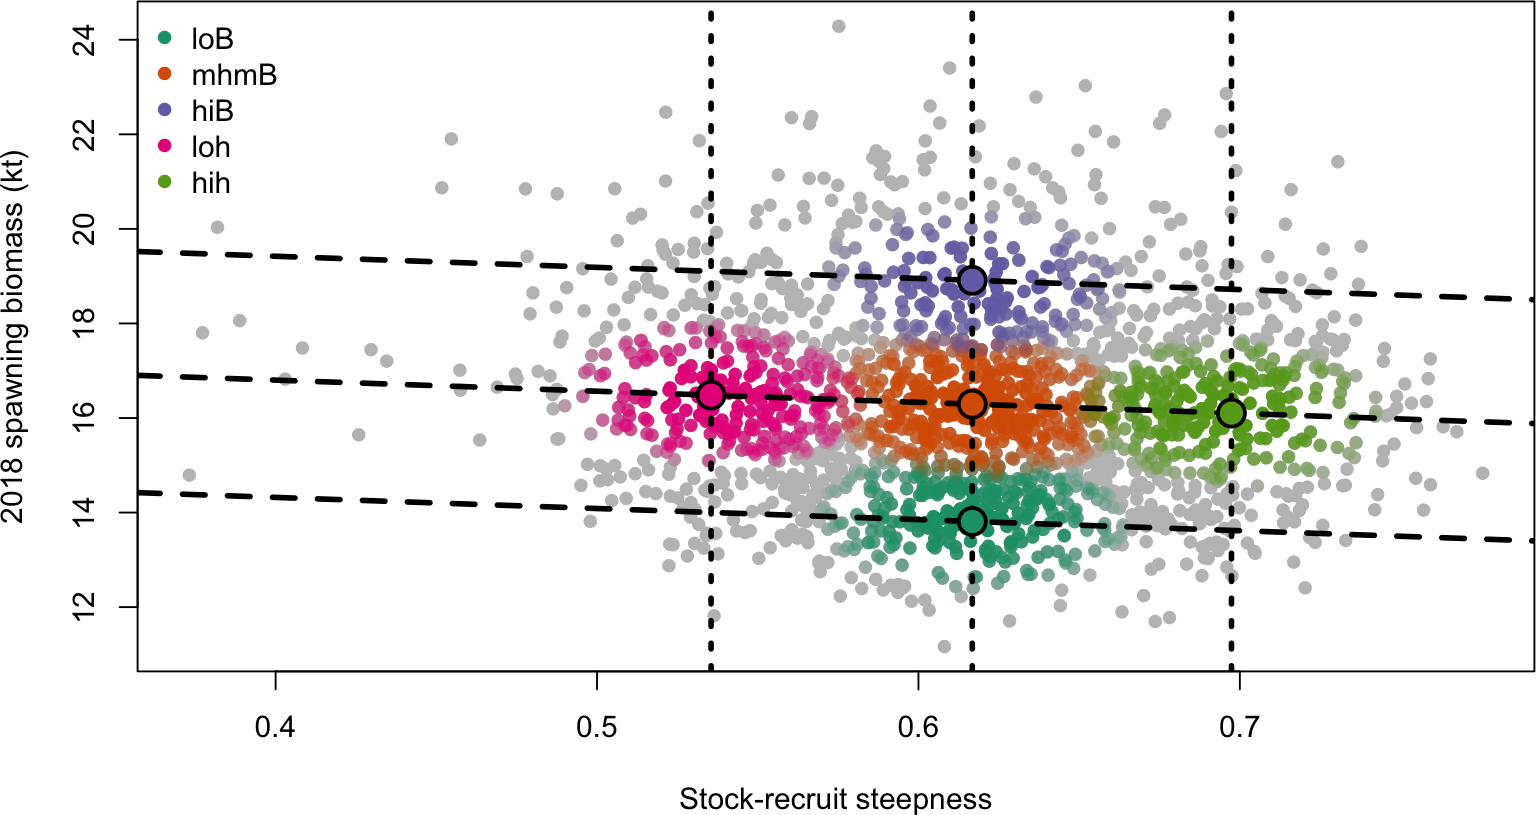
\includegraphics[width=0.9\linewidth]{knitr-figs-pdfunnamed-chunk-15-1}}{Figure \ref{fig:unnamed-chunk-15}} 

}

\caption{Joint marginal posterior distribution MCMC samples (grey dots) for stock-recruit steepness ($h$) and spawning biomass in 2018 ($B_{2018}$). Dashed lines indicate the mean, 10th and 90th percentiles of each marginal distribution, with the percentiles of the spawning biomass distribution adjusted to match the regression line between the two marginal distributions. Coloured dots with black borders at the intersections of selected percentiles are the sample centres for the 5 productivity/biomass operating model scenarios, with the coloured posterior MCMC samples showing the set of all points within a Mahalanobis distance of .6 from the centre of the same colour.}\label{fig:unnamed-chunk-15}
\end{figure}
\begin{figure}[htb]

{\centering \pdftooltip{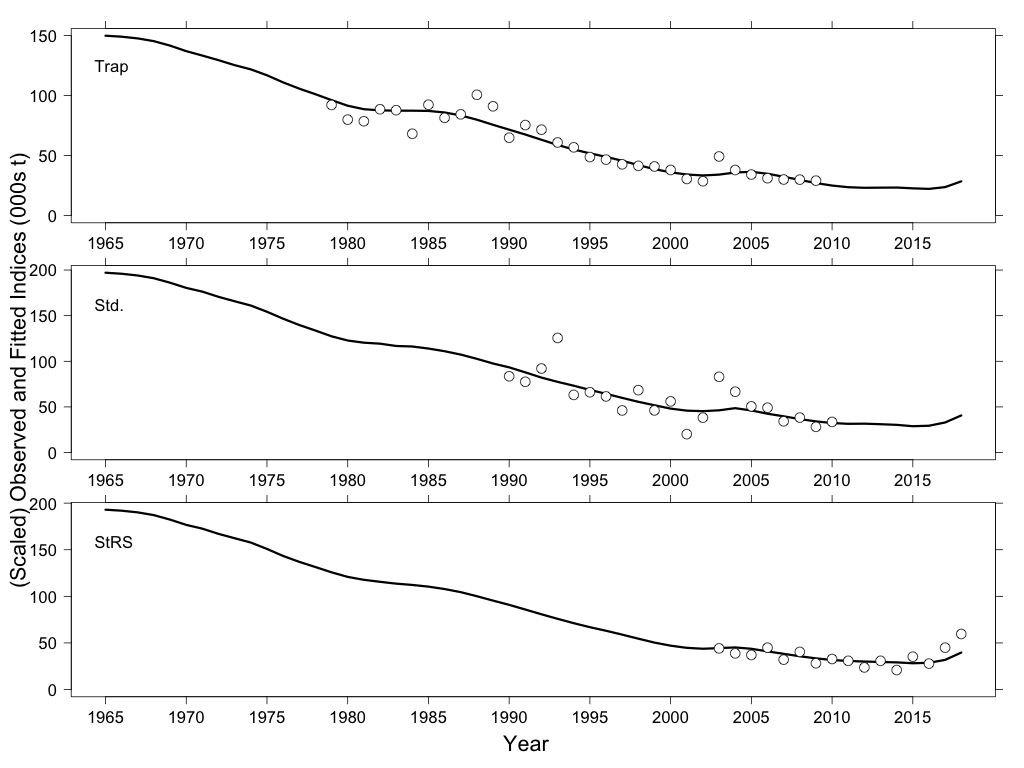
\includegraphics[width=0.9\linewidth]{data/base_ALK_mUnsexed/plotMLEindices}}{Figure \ref{fig:unnamed-chunk-16}} 

}

\caption{Operating model fits to Catch per Unit of Effort (CPUE) indices (kg/trap) from the commercial trap fishery (Trap, top), standardized sablefish survey (Std., middle), and stratified random sablefish survey (StRS, bottom). Points show observations scaled by catchability, and lines show operating model vulnerable biomass.}\label{fig:unnamed-chunk-16}
\end{figure}
\newpage
\begin{figure}[htb]

{\centering \pdftooltip{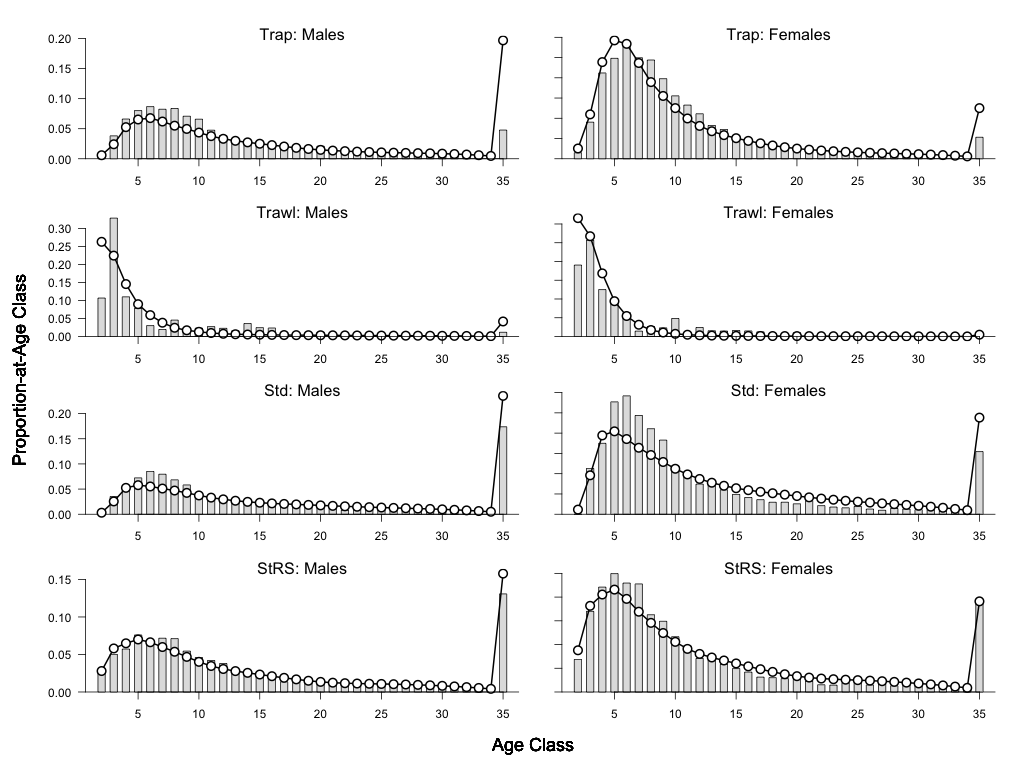
\includegraphics[width=0.9\linewidth]{data/base_ALK_mUnsexed/plotFitAgeFreq_avg}}{Figure \ref{fig:unnamed-chunk-17}} 

}

\caption{Averaged operating model fits to age observations for, from top to bottom, the commercial trap fishery (Trap), commercial trawl fishery (Trawl), standardized survey (Std.), and stratified random survey (StRS). Grey bars are the average proportion of age observations, and the points joined with a line show the average expected distribution of age observations in the operating model. Averages are taken over the years with observations.}\label{fig:unnamed-chunk-17}
\end{figure}
\newpage

\newpage
\begin{landscape}
\begin{figure}[htb]

{\centering \pdftooltip{\includegraphics[width=0.9\linewidth]{data/BtFitUtRt/hiRec2016_wtd/SP_hstAl_am5/BtFitUtRt_rep13}}{Figure \ref{fig:unnamed-chunk-19}} 

}

\caption{A single simulation replicate drawn from the reference set of operating models with the high estimated 2015 year class. The top row of panels show the spawning biomass (red line), legal biomass (black dashed line), and surplus production model estimated biomass (green and grey lines) when estimated as part of an MP. The middle row shows the legal (black solid line) and sub-legal (blue dotted line) harvest rates, and the bottom row shows the OM recruitments (black line with orange points).}\label{fig:unnamed-chunk-19}
\end{figure}
\newpage
\begin{figure}[htb]

{\centering \pdftooltip{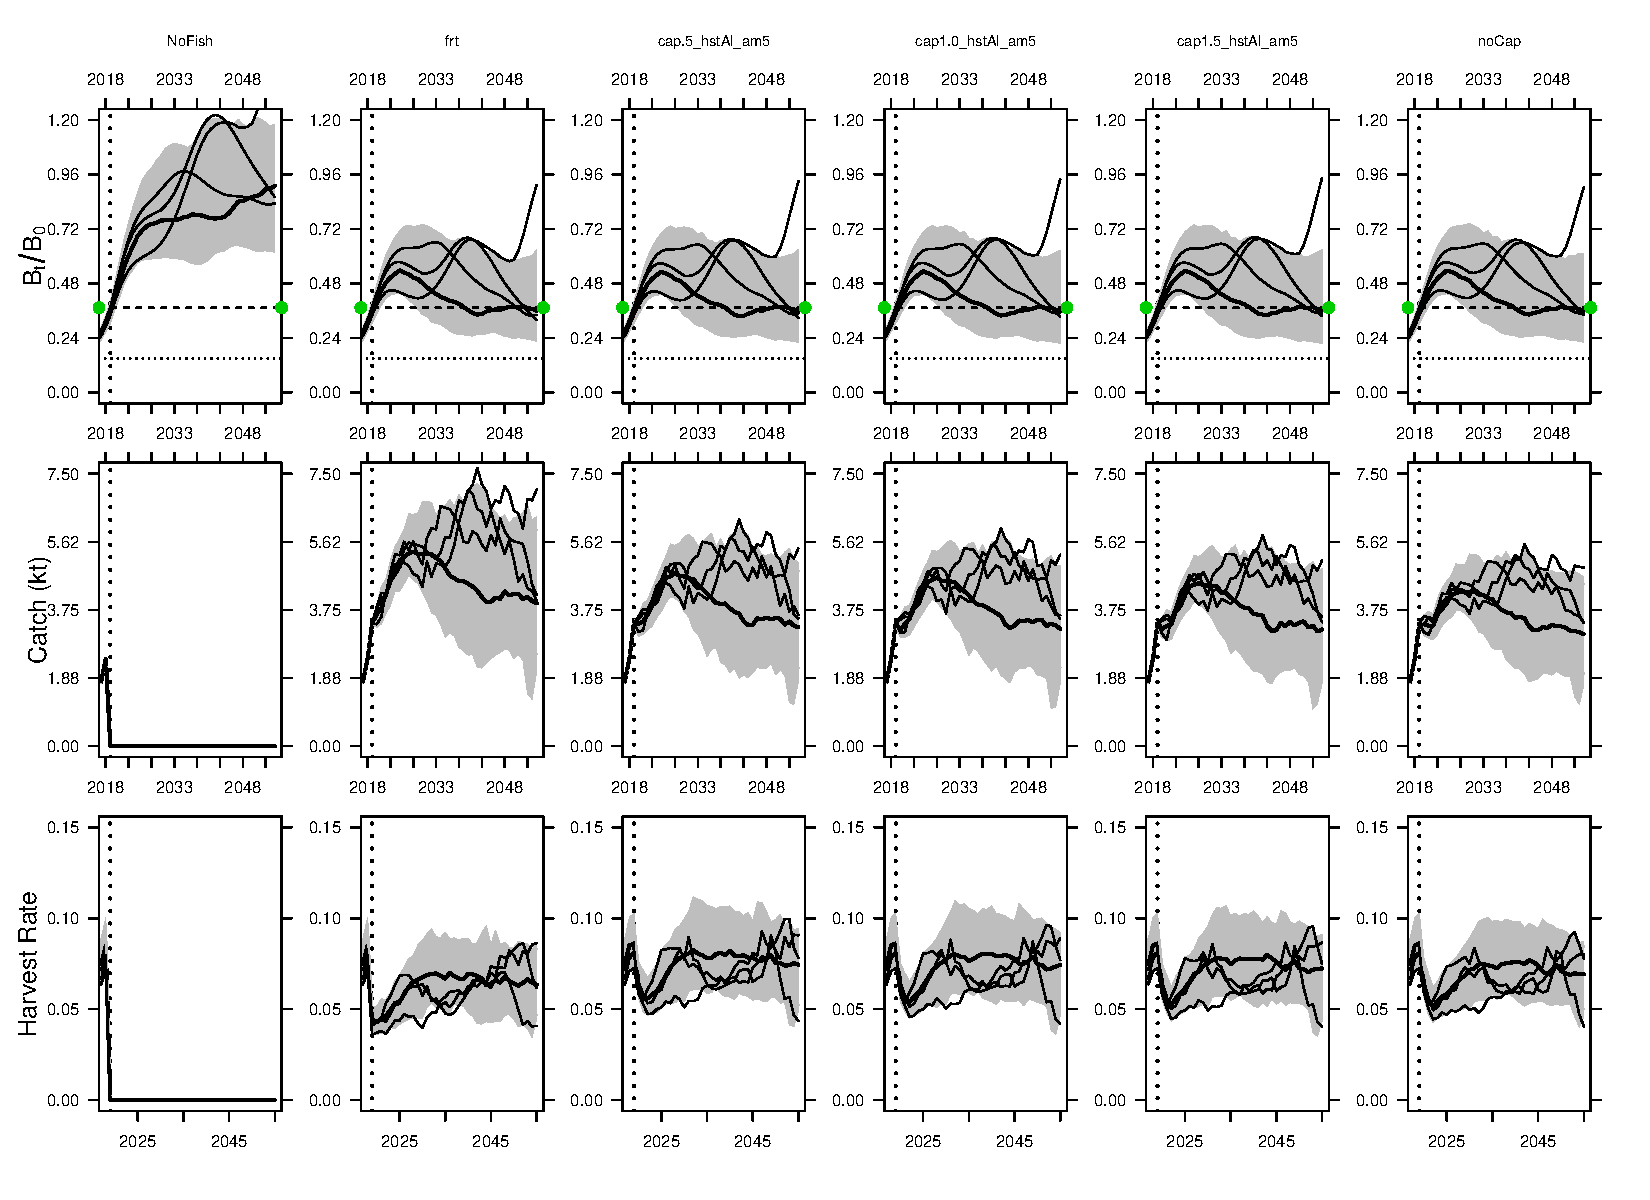
\includegraphics[width=0.9\linewidth]{data/tulipPlots/hiRec2016_wtd/depCatchHR/hiRec2016_wtd_depCatchHR_SP_hstAl_am5}}{Figure \ref{fig:unnamed-chunk-21}} 

}

\caption{Weighted combined simulation envelopes from the 5 productivity and biomass operating models in the reference recruitment scenario, showing management procedures that applied the historical allocation of discarding, and amortized overages over 5 years. The top row shows projected biomass relative to unfished, the second row shows the landed catch, and the bottom row shows the legal harvest rate.}\label{fig:unnamed-chunk-21}
\end{figure}
\newpage
\begin{figure}[htb]

{\centering \pdftooltip{\includegraphics[width=0.9\linewidth]{data/BtFitUtRt/simRec2016_wtd/SP_hstAl_am5/BtFitUtRt_rep13}}{Figure \ref{fig:unnamed-chunk-22}} 

}

\caption{A single simulation replicate drawn from the robustness set of operating models with a stochastically simulated 2015 year class. The top row of panels show the spawning biomass (red line), legal biomass (black dashed line), and surplus production model estimated biomass (green and grey lines) when estimated as part of an MP. The middle row shows the legal (black solid line) and sub-legal (blue dotted line) harvest rates, and the bottom row shows the OM recruitments (black line with orange points).}\label{fig:unnamed-chunk-22}
\end{figure}
\newpage
\begin{figure}[htb]

{\centering \pdftooltip{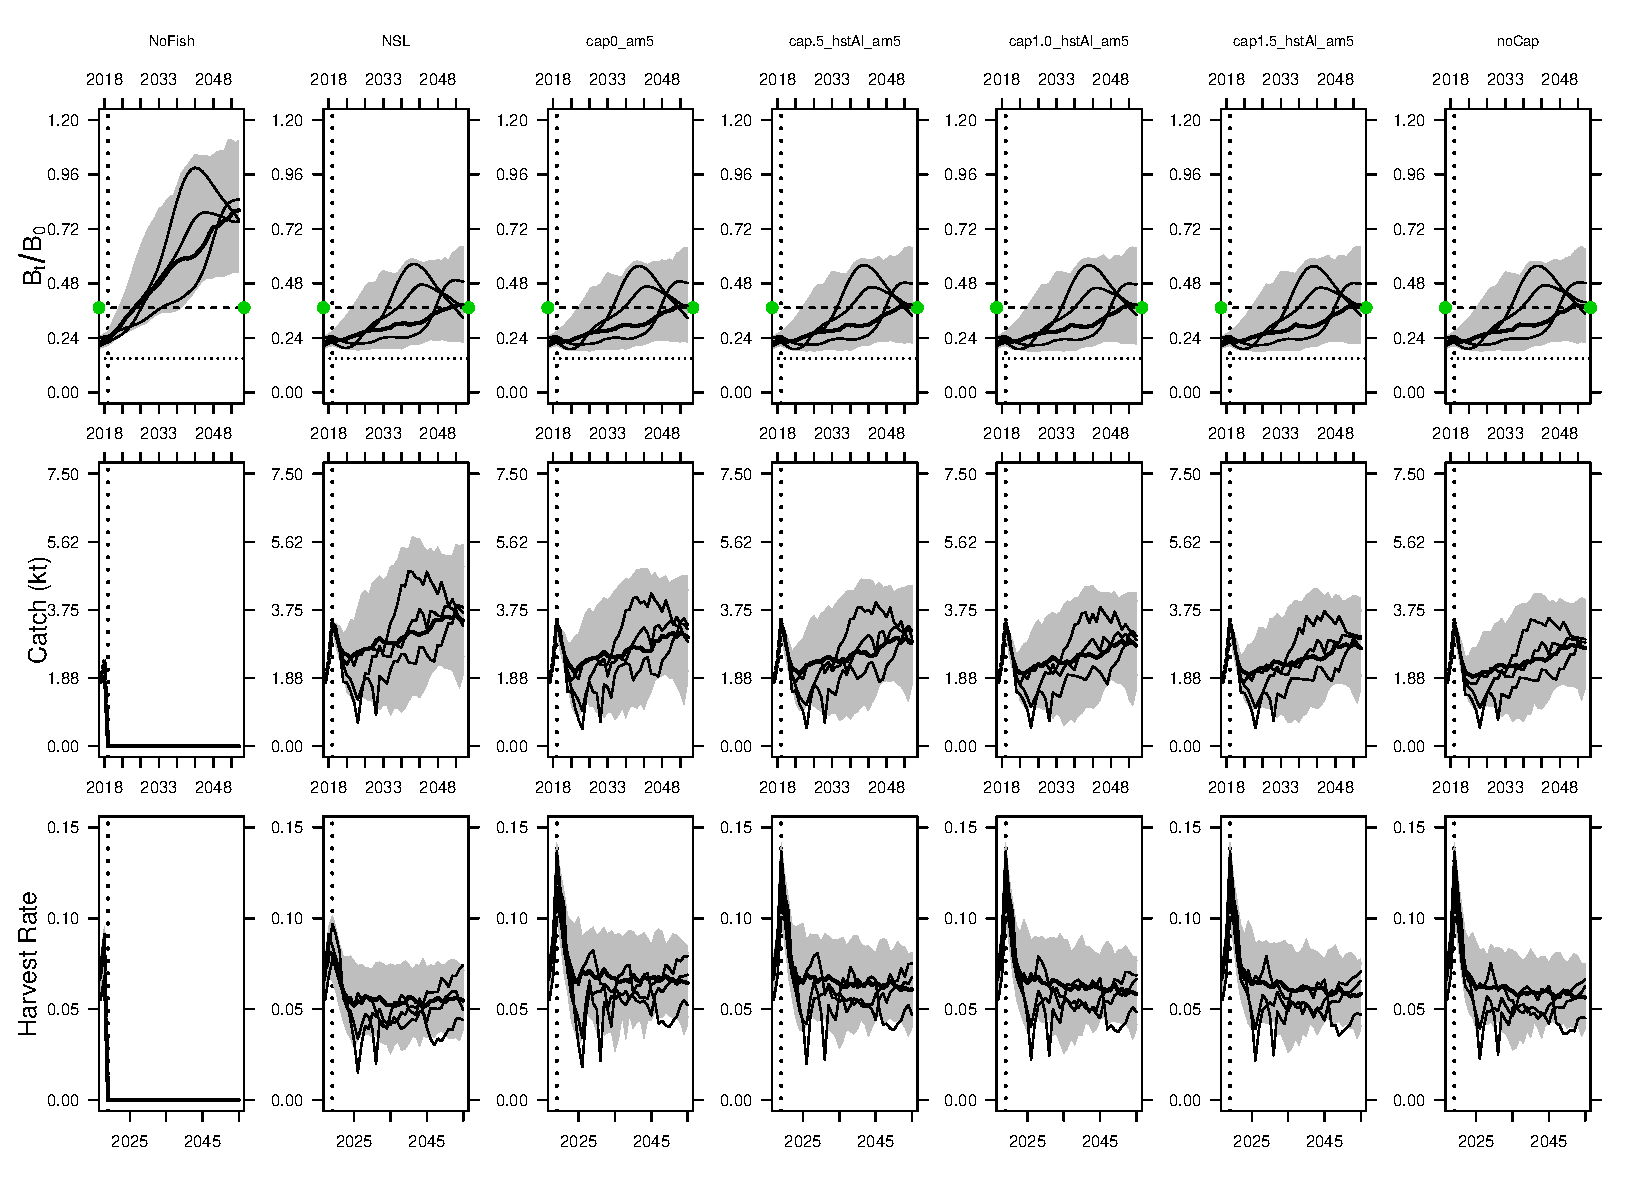
\includegraphics[width=0.9\linewidth]{data/tulipPlots/simRec2016_wtd/depCatchHR/simRec2016_wtd_depCatchHR_SP_hstAl_am5}}{Figure \ref{fig:unnamed-chunk-23}} 

}

\caption{Weighted combined simulation envelopes from the 5 productivity and biomass operating models in the robustness recruitment scenario, showing management procedures that applied the historical allocation of discarding, and amortized overages over 5 years. The top row shows projected biomass relative to unfished, the second row shows the landed catch, and the bottom row shows the legal harvest rate.}\label{fig:unnamed-chunk-23}
\end{figure}
\end{landscape}
\MakeAvailable

\end{document}
